\documentclass[a5paper,10pt]{scrbook}

\usepackage{musluatex}      % musicología pichicatiáo con -4.5ex en ejemplos ly en línea
\usepackage{graphicx}       % imágenes
\usepackage{caption}        % enlaza sobre la figura o el cuadro
\usepackage{float}          % para anclar flotantes (figuras y tablas) al lugar con opción [H]
\usepackage{tablefootnote}  % para \footnote{} en tabular
\usepackage{booktabs}       % tablas estéticas
\usepackage{multirow}       % filas múltiples en tablas
%\usepackage{fancyhdr}       % encabezado de páginas
%\pagestyle{fancy}
\usepackage[
  hidelinks,
  colorlinks=false,
  final,
  unicode,
  pdftitle={Análisis de una pieza inédita de Gustavo «Cuchi» Leguizamón},
  pdfauthor={Pablo Herrera},
]{hyperref}

%Apéndices
\usepackage[toc,page]{appendix}
\renewcommand{\appendixname}{Apéndices}
\renewcommand{\appendixtocname}{Apéndices}
\renewcommand{\appendixpagename}{Apéndices}

% Líneas viudas y huérfanas
\clubpenalty=10000
\widowpenalty=10000

\begin{document}
\title{Análisis de una pieza inédita de\\Gustavo «Cuchi» Leguizamón}
\subtitle{Himno a la Universidad Nacional de Salta}
\author{Pablo Herrera}
\date{\today}
\maketitle

\frontmatter
\newpage{\ }
\begin{center}
\vspace{2cm}

\textsc{Pablo Herrera}

\vspace{4cm}

\textbf{\LARGE Análisis de una pieza inédita de\\ Gustavo «Cuchi» Leguizamón}

\vspace{1cm}

\textbf{\large Himno a la Universidad Nacional de Salta}

\vspace{3cm}


\includegraphics[width=2cm]{img/escudo_unsa}

UNIVERSIDAD NACIONAL DE SALTA
\end{center}



\tableofcontents
\chapter{Prólogo}
\label{cap:prologo}

La propuesta original\footnote{Expediente ingresado el 24 de febrero de 2023 a horas 16:00 bajo el título \emph{Propuesta para una pericia de una melodía atribuida a Gustavo «Cuchi» Leguizamón}.} elaborada por mí para la \textsc{Universidad Nacional de Salta} para hacer una pericia sobre una línea melódica presente en la memoria de uno de los hijos del compositor salteño \textsc{Gustavo «Cuchi» Leguizamón} se vio necesariamente modificada cuando, por acción de la licenciada \textsc{Lucrecia Coscio}\footnote{\textsc{Lucrecia Coscio} es coordinadora del \textsc{Centro Cultural Holver Martínez Borelli}, dependiente de la Secretaría de Extensión Universitaria de la UNSa. }, se encontró una caja con documentación relacionada con el concurso para la letra de un himno a la Institución que la Universidad había llevado a cabo hace más de cuarenta años. En tal documentación, entre otras, se halló una partitura que, en parte, respondía a lo que \textsc{Juan Martín Leguizamón}, hijo del compositor, nos había ya referido como la melodía del \emph{Himno a la Universidad Nacional de Salta} que su padre había compuesto. Lo que en principio iba a ser un análisis de las estructuras subyacentes e intermedias\footnote{\emph{Estructuras subyacentes e intermedias} son términos propios de las técnicas de análisis schenkeriano.} de dicha melodía y de las posibles formas de armonizarla, pasó, obligadamente, a ser el análisis de una partitura en la que las armonías están completamente definidas y la línea melódica coincide solamente en forma parcial a lo aportado por el hijo del «Cuchi». Esas diferencias ---sin dudas significativas--- representan una oportunidad para poder mostrar un aspecto poco conocido de la obra de Leguizamón: su obra musical no son solamente zambas y chacareras en compás de \hbox{\compas{6}{8}(\compas{3}{4}).}\footnote{El compás de \hbox{\compas{6}{8}(\compas{3}{4}).} es el patrón rítmico complejo de mucha música latinoamericana que combina tanto en la sucesión como en la simultaneidad patrones de dos pulsos (\compas{6}{8}) y tres pulsos(\compas{3}{4}).} A la vez también es una oportunidad para reflexionar mínimamente sobre lo que se ---y lo que no es--- la memoria.

La partitura encontrada con la documentación referente al concurso de 1982 organizado por la Universidad \emph{para elegir una letra} para el futuro Himno ---concurso que al igual que el celebrado un año antes fuera declarado desierto--- contiene la letra del concursante que se presentara con el seudónimo \textsc{Budotizo}. Al no ser esta letra ganadora del concurso, con criterio que compartimos plenamente, las actuales autoridades de la Institución piensan en una nueva letra. Para tal fin se nos hace necesario analizar tanto las acentuaciones y la forma musical en relación a las acentuaciones y la forma de esta poesía como así también advertir de las divergencias entre los acentos musicales y poéticos que en una letra bien confeccionada para esta música no deben estar.

El \textsc{«Cuchi» Leguizamón}, en conocida entrevista televisiva y  con lenguaje coloquial, nos revela parte de su pensamiento musical, consistente en incluir en la simultaneidad dos enfoques de un mismo objeto, algo que en técnica de composición se conoce como \emph{bitonalidad}. Hemos considerado que en el marco del presente informe cabía desarrollar un capítulo de carácter más técnico, que con seguridad requiere de altas competencias en teoría musical para abordar con total profundidad su lectura, y no sólo cabía sino que hasta necesario se hace, aunque más no sea en ciertos límites, mostrar en términos teóricos lo que de las obras musicales de Leguizamón se desprende como pensamiento y recurso expresivo.

La valoración del hallazgo y rescate de una pieza de uno de los más emblemáticos compositores de la cultura de Salta y la presentación de  posibilidades futuras sobre ella cierran este informe que entre otras cosas nos ha permitido \emph{empezar} a poner en palabras un tanto más rigurosas el modo de hacer de una mente brillante y un espíritu inspirado: la mente y el espíritu de \textsc{Gustavo «Cuchi» Leguizamón}.

\chapter{Algunas convenciones de escritura
musical}
\label{pre:convenciones}

\section*{Grados}

Para los grados melódicos hemos adoptado le convención schenkeriana: números arábigos para los grados melódicos y números romanos para los grados armónicos.

\begin{table}[H]
\centering
\begin{tabular}{@{}lll@{}}
\toprule
\textbf{Grado} & \textbf{Melódico}  & \textbf{Armónico} \\
\midrule
Primer grado   & \grado{1}          & I                 \\
Segundo grado  & \grado{2}          & II                \\
Tercer grado   & \grado{3}          & III               \\
Cuarto grado   & \grado{4}          & IV                \\
Quinto grado   & \grado{5}          & V                 \\
Sexto grado    & \grado{6}          & VI                \\
Séptimo grado  & \grado{7}          & VII               \\
Octavo grado   & \grado{8}          & ---              \\
\bottomrule
\end{tabular}
\caption*{Grados.}\label{pretab:grados}
\end{table}

El bajo en los grados armónicos se escribe como subíndice bajo el grado (en romano) o el nombre de la fundamental. Las notas añadidas a la triada se escriben como superíndice. Ejemplo: la dominante séptima del segundo grado con su tercera alterada en el bajo se cifra \acorde.V.\sostenidotxt3.7.../II, y, en la tonalidad de Fa mayor, también se puede escribir como \acorde.Re.Fa\sostenidotxt.7....

\section*{Ligaduras}

La ligadura semipunteada significa dependencia de la primera respecto a la segunda nota. Ejemplo:

\begin{figure}[H]
\centering
\begin{lilypond}[notime]
\relative {
  \hide Stem
  \slurHalfDashed
  e''4 ( c2 ) \bar "||"
  \slurHalfSolid
  e,2 ( g4 ) \bar "||"
}
\end{lilypond}
\caption*{Dependencia de una nota.}\label{prefig:dependencia}
\end{figure}

Las ligaduras punteadas se utilizan para marcar \emph{puentes de segundas}. Ejemplo:

\begin{figure}[H]
\centering
\begin{lilypond}
\relative {
  \time 2/4
  \tempo "Tempo di ritorno"
  \partial 8
  f''16 g
  \slurDashed
  a4. ( g16 f g8 ) ( e4 e8
  f4. ) ( e16 d e8 )
}
\end{lilypond}
\caption*{Puente de segundas.}
\label{prefig:puente}
\end{figure}

\mainmatter
\chapter{Memorias}
\label{cap:memorias}

La memoria es un acto en el presente. En tal acto, tanto la imaginación como las experiencias, las competencias, las necesidades, los intereses, las emociones, los sentimientos y los sesgos personales no pueden no influir. Las expectativas personales y sociales también pesan en el presente acto de recordar. \emph{Recordar} es volver a pasar por el corazón, \emph{recordar} es volver a sonar. Con esto en mente, con la conciencia de que recordar es un acto creativo, intento traer a mi memoria tanto la primer reunión con las autoridades universitarias como la reunión entre «Pajarito», Juan Martín y yo.


\section{El canto y las palabras de un hijo}
\label{sec:palabra-canto}

\begin{figure}[H]
\centering
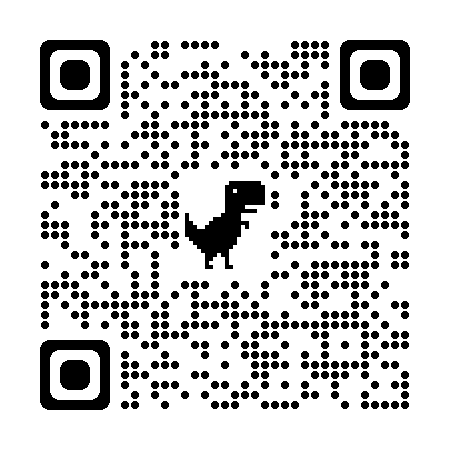
\includegraphics[width=0.3\textwidth]{img/qrcode-himno-memoria}
\caption{El canto y las palabras de \textsc{Juan Martín Leguizamón}.}
\label{fig:canto-palabras}
\end{figure}


En diciembre de 2022 me contacta \textsc{Marcelo «Pajarito» Sutti}\footnote{\textsc{Marcelo Sutti} es destacado poeta y músico salteño.}, quien me informa que \textsc{Juan Martín Leguizamón}\footnote{\textsc{Juan Martín Leguizamón}, hijo de Gustavo, es antropólogo y presidente de la Fundación Legado Cultural Cuchi Leguizamón.} le refiere tener viva en su memoria una melodía que recuerda bajo el título de \emph{Himno a la UNSa}. Enteradas las autoridades de la Universidad del relato de Juan Martín ---y mediado por Sutti quien me señala ante ellas como un hombre idóneo para realizar un peritaje sobre la melodía en memoria del hijo del «Cuchi»---, organizan una reunión en la que acordamos trabajar sobre el fragmento recordado y su posible relación con los modos de componer del legendario músico saleño. La posibilidad de establecer un grado de compatibilidad entre la melodía a estudiar y las melodías de Gustavo Leguizamón existe porque existen técnicas de análisis que pueden develar estructuras análogas en diversas piezas de un mismo autor. El \emph{análisis schenkeriano} en el particular caso me pareció una herramienta adecuada por ser capaz de mostrar estructuras intermedias y de superficie propias de un autor es específico, y es la que propuse en esa reunión utilizar en la pericia.

No recuerdo si primero fue la reunión con las autoridades universitarias, o si antes fue la reunión con Sutti y Leguizamón (h). No importa\footnote{La reunión con Sutti y Leguizamón (h) fue el 20 de diciembre de 2022 en mi domicilio particular y la grabación fue registrada a las 16:46 horas; con las autoridades nos reunimos el día 27 del mismo mes a las 16:00 horas en un bar del centro de la ciudad de Salta.}. Sí importa que fue una tarde de verano con un cielo tapado de amenazantes y negras nubes. El momento central de esa amena y nada amenazante charla no es necesario recordarlo: el registro electrónico nos exime del acto creativo de recordar, y él es accesible con el código QR de la Figura~\ref{fig:canto-palabras}.

\begin{figure}[htb]
\begin{ly}
\relative {
  \clef "treble"
  \key es \major
  \time 12/8
  \tempo 4.= 55
  \partial 8
  bes8
  es4. ~ es4 es8 es4 c8 ~ c d es
  f4. ~ f8 f es d4. r4 bes8
  g'4. ~ g4 g8 g4 es8 ~ es f g
  aes4. aes8 aes g f4. r4 bes8
  es4. ~ es4 es8 es4 c8 ~ c d es
  d4. ~ d8 bes g bes4. r
  c8 aes4 ~ aes aes8 aes f4 ~ f8 g aes
  g4. ~ g4 g8 g4 es8 ~ es f g
  f4. ~ f8 g f c4 d bes
  es4.
}
\end{ly}
\caption[Transcripción de un fragmento de la melodía recordada.]{Transcripción de la melodía recordada y cantada por \textsc{Juan Martín Leguizamón.}}
\label{fig:Transcripcion}
\end{figure}

Basta con transcribir un fragmento de lo cantado por el hijo del «Cuchi» para detectar una serie de significativas características, algunas que acercan esta versión a la versión escrita (mostrada y estudiada en el Capítulo~\ref{cap:partitura}), otras que producen la divergencia entre ellas.

La tonalidad de Mi\bemoltxt mayor utilizada por Juan Martín ---a diferencia de la de Fa mayor consignada en la partitura--- es debido a que para su registro de voz ---y no sólo para el de él, sino para el registro vocal de la mayoría de la población--- esta tonalidad es más conveniente. La melodía escrita por su padre, en Fa mayor, es de difícil canto para la mayoría de la etnia de Salta. Sin embargo, en amplio pasaje las dos versiones coinciden en su conformación interválica, reconociéndose en la versión de Juan Martín la pieza de Gustavo Leguizamón. A tal punto es así que el 23 de abril de 2023 a la tarde, consultado yo telefónicamente por \textsc{Lucrecia Coscio}\footnote{Coordinadora del Centro Cultural Holver Martínez Borelli de la UNSa.} acerca de si algunas de las partituras que me enviaba vía \emph{WhatsApp} tenía relación con la melodía referida por Juan Martín.

\begin{figure}[htb]
\centering

\includegraphics[width=0.4\textwidth]{img/lucrecia1}
\caption{21 de abril: hallazgo de la partitura.}
\label{fig:hallazgo-partitura}
\end{figure}

\noindent Ese mismo día, en horas de la mañana, la profesora Coscio me había enviado otras partituras que indudablemente no tenían relación con la melodía en cuestión, y así lo hice saber. Pero faltando 12 minutos para las 19:00 horas, Lucrecia vuelve a comunicarse conmigo. Mientras me dirijo a la presentación de la flamante \emph{Fundación Legado Cultural Cuchi Leguizamón} veo las fotos y reconozco de inmediato el parentesco de lo que está escrito con lo cantado durante una tormenta de verano cuatro meses atrás: es el himno del «Cuchi»\footnote{Esa misma tarde, junto a la partitura se halló un sobre conteniendo los datos de los autores de la letra y la música (ver Figura~\ref{fig:sobre-letra} en la página~\pageref{fig:sobre-letra}).}. Gol.


\section{La memoria oral y la memoria escrita}
\label{sec:memoria-oral-escrita}

En la escritura musical la representación de las alturas de los sonidos no reviste ambigüedad alguna debido a que el sistema musical convencional ---el usado por Leguizamón--- consiste en doce notas afinadas en el temperamento igual, representadas gráficamente con cabezas de notas ubicadas más arriba o más abajo sobre un pentagrama que es presidido por una clave que indica registro agudo (clave de sol), medio (claves de do) o grave (clave de fa). El ritmo, basado en figuras organizadas en sistema binario\footnote{Al ser una \blanca\ la representación de una duración que es la mitad de una \redonda, la \negra\ la mitad de una \blanca, la \corchea\ la mitad de una \negra, la \semicorchea\ la mitad de una \corchea, etc., queda evidenciado que el sistema utilizado para la representación de duraciones es \emph{binario}.}, tiene limitaciones respecto a la flexibilidad con la que los seres humanos solemos tratar, a la hora de la interpretación, al ritmo musical. Sin embargo, la representación rítmica en una partitura bien escrita acerca, y mucho, la idea rítmica que un compositor tiene \emph{in mente} o en su propia experiencia interpretativa de una obra. Dicho de otro modo: si se ejecuta una partitura rígidamente, matemáticamente, se puede percibir esa interpretación como algo «deshumanizada», pero nunca muy lejos de la idea rítmica que el compositor tuvo al anotarla.

\begin{figure}[htb]
\begin{ly}
\relative {
  \key es \major
  \time 2/4
  \partial 8
  bes8
  es4. es8
  es c d es
  f4 f8 es
  d4. bes8
  g'4. g8
  g es f g
  aes4 aes8 g
  f4. bes8
  es4. es8
  es c d es
  d4 bes8 g
  bes4. c8
  aes4 aes
  aes4. bes8
  g f g es
  f c d bes
  es4.
}
\end{ly}
\caption{Fragmento de la partitura del \emph{Himno} transportado a Mi\bemoltxt mayor.}
\label{fig:frag-partitura}
\end{figure}

Volvamos por unos instantes al fragmento transcripto de la versión oral de Juan Martín Leguizamón (Figura~\ref{fig:Transcripcion}, página~\pageref{fig:Transcripcion}). Si la comparamos en el aspecto melódico con la versión escrita por su padre y transcripta a Mi\bemoltxt\ mayor\footnote{Originalmente en Fa mayor, transscribimos a Mi\bemoltxt a los fines de facilitar la comparación con el fragmento cantado.} en la Figura~\ref{fig:frag-partitura}, notamos que hasta el compás 12 de la versión escrita (compás 6 de la versión oral) hay plena coincidencia, pero a partir de compás 13 (compás 7 de la Figura~\ref{fig:Transcripcion}) la divergencia entre ambas versiones es más que clara. A partir de ahí, la versión oral construye un puente de segundas \musncp{\key es \major aes'2 g' f' es'} también presente en la versión escrita, pero sin la aceleración cronométrica\footnote{La aceleración cronométrica está dada par la presencia creciente de corcheas que generan en la percepción del oyente una especie de apuro respecto a lo precedente que es vivido como una aceleración, aunque el \emph{tempo} permanezca inmutable.} existente en la versión escrita y con regularidades rítmicas que hacen al fragmento más inocente y menos elaborado.

Desde el pundo de vista rítmico, las diferencias entre los fragmentos de las Figuras~\ref{fig:Transcripcion} y \ref{fig:frag-partitura} son definitivamente inmensas: la versión oral, en \compas{12}{8}, tiene al pulso subdividido en tres, lo que asemeja esta versión a la rítmica usada mayoritariamente en las formas de danza de apariencia más folclórica de Leguizamón (zambas, chacareras, etc.). Lo escrito y presentado en el concurso de 1982, en compás de \compas{2}{4}, subdivide el pulso en dos, alejándose radicalmente del carácter rítmico impreso en la versión oral de la pieza, acercándose, por el compás que usa, a los códigos musicales empleados tradicionalmente en los himnos del mundo y alejándose el autor de su más habitual práctica rítmica. En este sentido, cobra especial valor el relato de Juan Martín, hacia el final de la grabación (ver, escanear la Figura~\ref{fig:canto-palabras} y oír), donde recobra la palabra de su padre afirmando que algo de una marcha de caballería tiene este himno, marcha de caballería que de ninguna manera podría estar en un compás compuesto, sino en el compás simple en el que está presentada la partitura.

En el mes de julio de 2023 recibo la visita de Juan Martín, quien trae consigo un par de manuscritos de su padre que sirven para comarar y constatar su caligrafía musical (Figur~\ref{fig:manuscritos}). Aprovechamos la ocasión para oír la maqueta (Figura~\ref{fig:grabacion}, página~\pageref{fig:grabacion}) de la partitura hallada en abril (Apéndice en la página~\pageref{apx:partitura}). La impresión que tiene en ese momento Juan Martín es la de encontrar «my rígida» la versión de computadora y no termina de reconocer lo recordado por él en dicha versión. Atribuye tal rigidez a la precisión deshumanizada de la computadora. Sin embargo, cuando le hago oír la maqueta de la transcripción que hice de su versión cantada, ya no le parece que la computadora sea rígida tocando, y sí se identifica con lo oído.

Por todo lo mostrado y argumentado anteriormente, no dudamos que sin el testimonio de Juan Martín Leguizamón no se podría haber transitado de igual forma el camino del invaluable rescate de una compasición de Gustavo Leguizamón, y tampoco dudamos que la partitura encontrada por Lucrecia Coscio es la memoria más fiel de esa composición, partitura que revelamos en el Capítulo~\ref{cap:partitura} (página~\pageref{cap:partitura}), previa revisión de la letra y su relación con el ritmo musical, tratada en el Capítulo siguiente.

\section{La oralidad en la escritura}
\label{sec:oralidad-escritura}

Una de las memorias más valiosas con la que nos podemos encontrar en este enriquecedor proceso del rescate del \emph{Himno a la Universidad Nacional de Salta} de Gustavo Leguizamón es la de, una vez más en la obra musical del «Cuchi», hallar representada el habla salteña en las líneas melódicas de esta canción hecha himno. No es menor el dato: un himno sin forma do himno, un himno sin estribillo, un himno con forma de canción, con frases musicales de perfil poético y no prosaico. Un ícono de la cultura de Salta que esperó más de cuarenta años para ver la luz, dormido en una carpeta de un frío archivo universitario y soñado en la memoria viva de los hijos de su compositor. Hoy despierta, sale a la luz, quizás ---ojalá--- para finalmente cumplir con la intención autoral de hacerse \emph{Himno} de la Universidad Pública de su provincia.

\chapter{Letra y ritmo musical}
\label{cap:letra-ritmo}

\begin{figure}[H]
\centering
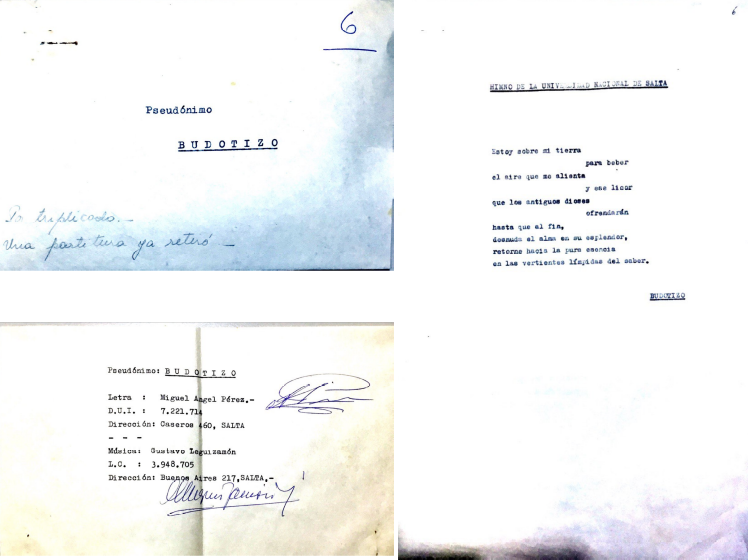
\includegraphics[width=0.6\textwidth]{img/sobre-seudonimo-poema}
\caption{Sobre, datos del seudónimo y letra del Himno.}
\label{fig:sobre-letra}
\end{figure}

\section{Himno a la Universidad Nacional de Salta}
\label{sec:himno-letra}

\texttt{ %\footnotesize
\begin{verse}
Estoy sobre mi tierra\\
\hspace{4cm}para beber\\
el aire que me alienta\\
\hspace{4cm}y ese licor\\
que los antiguos dioses\\
\hspace{4cm}ofrendarán\\
hasta que al fin,\\
desnuda el alma en su esplendor,\\
retorne hacia la pura esencia\\
en las vertientes límpidas del saber.
\end{verse}
\hspace{5cm} Miguel Ángel Pérez (1982)
}

\vspace{0.5cm}

En el Cuadro~\ref{tab:analisis-letra} realizamos un breve análisis de la métrica del poema. En él notamos, como datos sobresalientes, que Leguizamón eligió \emph{siempre} utilizar las sinalefas, e incluso eligió unir con una sinalefa los dos últimos versos, de nueve y once sílabas cada uno, quedando como consecuencia diecinueve sílabas entre los dos versos.

\begin{table}[H]
\centering
\rotatebox{90}
{
\begin{tabular}{@{}llll@{}}
\toprule
\multirow{2}{*}{Versos}                & \multicolumn{3}{c}{Sílabas}                  \\
                                       & sin sinalefas & con sinalefas & en la música \\
\midrule
Estoy sobre mi tierra {[} para beber   & 11            & 11            & 11           \\
el aire que me alienta {[} y ese licor & 13            & 11            & 11           \\
que los antiguos dioses {[} ofrendarán & 11            & 11            & 11           \\
hasta que al fin,                      & 5             & 4             & 4            \\
desnuda el alma en su esplendor,       & 11            & 8             & 8            \\
retorne hasta la pura esencia          & 11            & 9             & 9            \\
en las vertientes límpidas del saber.  & 11            & 11            & 11 (10)\tablefootnote{Los dos últimos versos soportan, al unirlos, una sinalefa entre ellos, que es usada por Leguizamón, haciendo así de los dos últimos un verso de diecinueve sílabas.}      \\
\bottomrule
\end{tabular}
}
\caption{Análisis silábico del poema de Miguel Ángel Pérez.}
\label{tab:analisis-letra}
\end{table}

\begin{table}[H]
\begin{minipage}{\textwidth}
\centering
\begin{tabular}{@{}ll@{}}
\toprule
ritmo-melodía-verso     & sílabas\footnote{Entre paréntesis anotamos las sílabas tal como se tienen en cuenta desde el pensamiento estrictamente literario, el cual contempla una sílaba más para versos terminados en acentuación aguda, mas nos quedamos con los números que coinciden con la cantidad de notas en el ritmo de la melodía.} \\
\midrule
\lilyfile{part/verso1}  & 11(12)  \\
\lilyfile{part/verso2}  & 11(12)  \\
\lilyfile{part/verso3}  & 11(12)  \\
\lilyfile{part/verso4}  & 4(5)    \\
\lilyfile{part/verso5}  & 8(9)    \\
\lilyfile{part/verso6}  & 19(20)  \\
\bottomrule
\end{tabular}
\end{minipage}
\caption[Resolución rítmico-melódica de la letra en la música.]{Resolución rítmico-melódica de la letra en la música.}
\label{tab:ritmo-letra}
\end{table}

El Cuadro~\ref{tab:ritmo-letra} aclara especialmente la resolución rítmico-melódica de los últimos cuatro versos de la letra, respetando en su unicidad el único verso de cuantro sílabas que posee el poema y, a continuación generando con los tres versos siguientes dos frases musicales de ocho y diecinueve sílabas respectivamente que proveen al final de la pieza de una asimetría que atenta contra el aburrimiento.

\begin{figure}[H]
\centering
\ritmo{\time 2/4 \partial 8 f8 f4. f8 f f f f f4 f8 f f4.}
\caption{Patrón rínmico predominante.}
\label{fig:patron-ritmico}
\end{figure}

El ritmo de la Figura~\ref{fig:patron-ritmico} es el patrón que marca todos los versos de once sílabas. La decisión compositiva de no continuar en los últimos tres versos con la métrica presente en el poema es fundamental a la hora de definir la estética de la pieza, ya que sin la ruptura de la simetría el sopor podría haberse adue;ado del final de esta canción.

Volviendo sobre el ritmo predominante en la pieza (Figura~\ref{fig:patron-ritmico}) esta vez en relación con la letra, debemos decir que en dos ocasiones sucede algo que es bastante habitual encontrar en la música popular: palabras acentuadas de manera diferente en la música a como son en el habla. La primera de éstas acontece entre los compases 1 y 2 \ritmoletra{\time 2/4 \partial 8 f8 f4. f8\upbow f\downbow f f f} {Es -- toy so -- bre la tie -- rra...}\footnote{Los símbolos \lilyGlyph{scripts.upbow} (punta) y \lilyGlyph{scripts.downbow} (talón) provienen de los conceptos de \emph{arsis} y \emph{thesis}, alzar y dar, al aire y a tierra, no acentuado y acentuado. El movimiento de un pie al caminar tiene esos dos momentos: no acentuado cuando se apoya sobre su punta, y acentuado cuando se apoya, en un nuevo paso, el talón. Los instrumentos de cuerda frotada heredan estos símbolos resignificándolos como punta y taco del arco e indican con qué parte del arco debe atacarse la nota señalada.} donde con la palabra \emph{sobre}, y la segunda, de forma análoga, sucede entre los compases 33 y 34 \ritmoletra{\time 2/4 \partial 8 f8 f4. f8\upbow f\downbow f f f} {re -- tor -- ne~ha -- cia la pu -- ra~e...} donde con la palabra \emph{hacia}, son acentuadas en forma aguda, siendo ellas, claramente, palabras de acentuación grave. Un tercer caso de cambio de acentuación se encuentra entre los compases 29 y 30 \ritmoletra{\time 2/4 \partial 8 f8\upbow f4\downbow f f4.}{has -- ta que~al fin...} donde \emph{hasta} es, por acción del ritmo musical, convertida en una palabra con acentuación aguda. Este último caso es aún más llamativo que los dos anteriores debido a que este cambio de acentuación sucede justo en donde el poema, en su verso central, tiene cuatro sílabas, métrica muy diferente a los endecasílabos anteriores y posteriores. en la música también es llamativo, en ese par de compases se utiliza el ritmo \ritmo{\time 2/4 \partial 8 8 4 4 4.} por única vez en toda la pieza.

Sólo queda mencionar una característica general del ritmo musical, que condiciona tanto a la letra de Pérez como a cualquier otra letra que se le quiera poner a este himno: las frases \emph{siempre} terminan en forma tética, es decir en tiempo fuerte, acentuadas, lo que exige en la letra análogo comportamiento, es decir versos con acentuación aguda.

\chapter{La partitura}
\label{cap:partitura}

\begin{figure}[H]
\centering
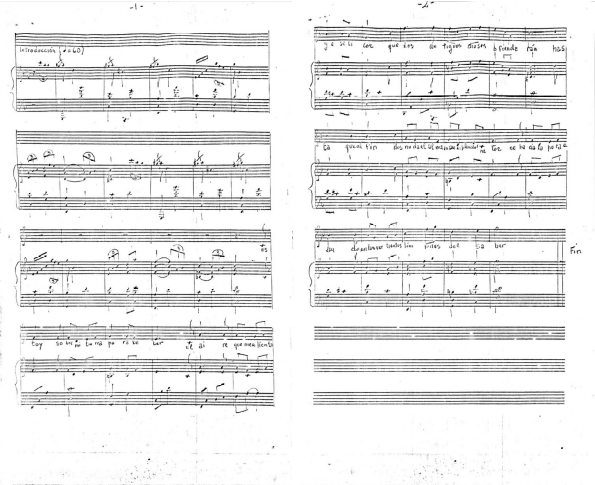
\includegraphics[width=1.0\textwidth]{img/partitura-original}
\caption{Copia del manuscrito del himno de Gustavo Leguizamón.}
\label{fig:partitura}
\end{figure}

\section{La caligrafía del manuscrito}
\label{sec:caligrafia}

\begin{figure}[H]
\begin{minipage}{\textwidth}
\centering
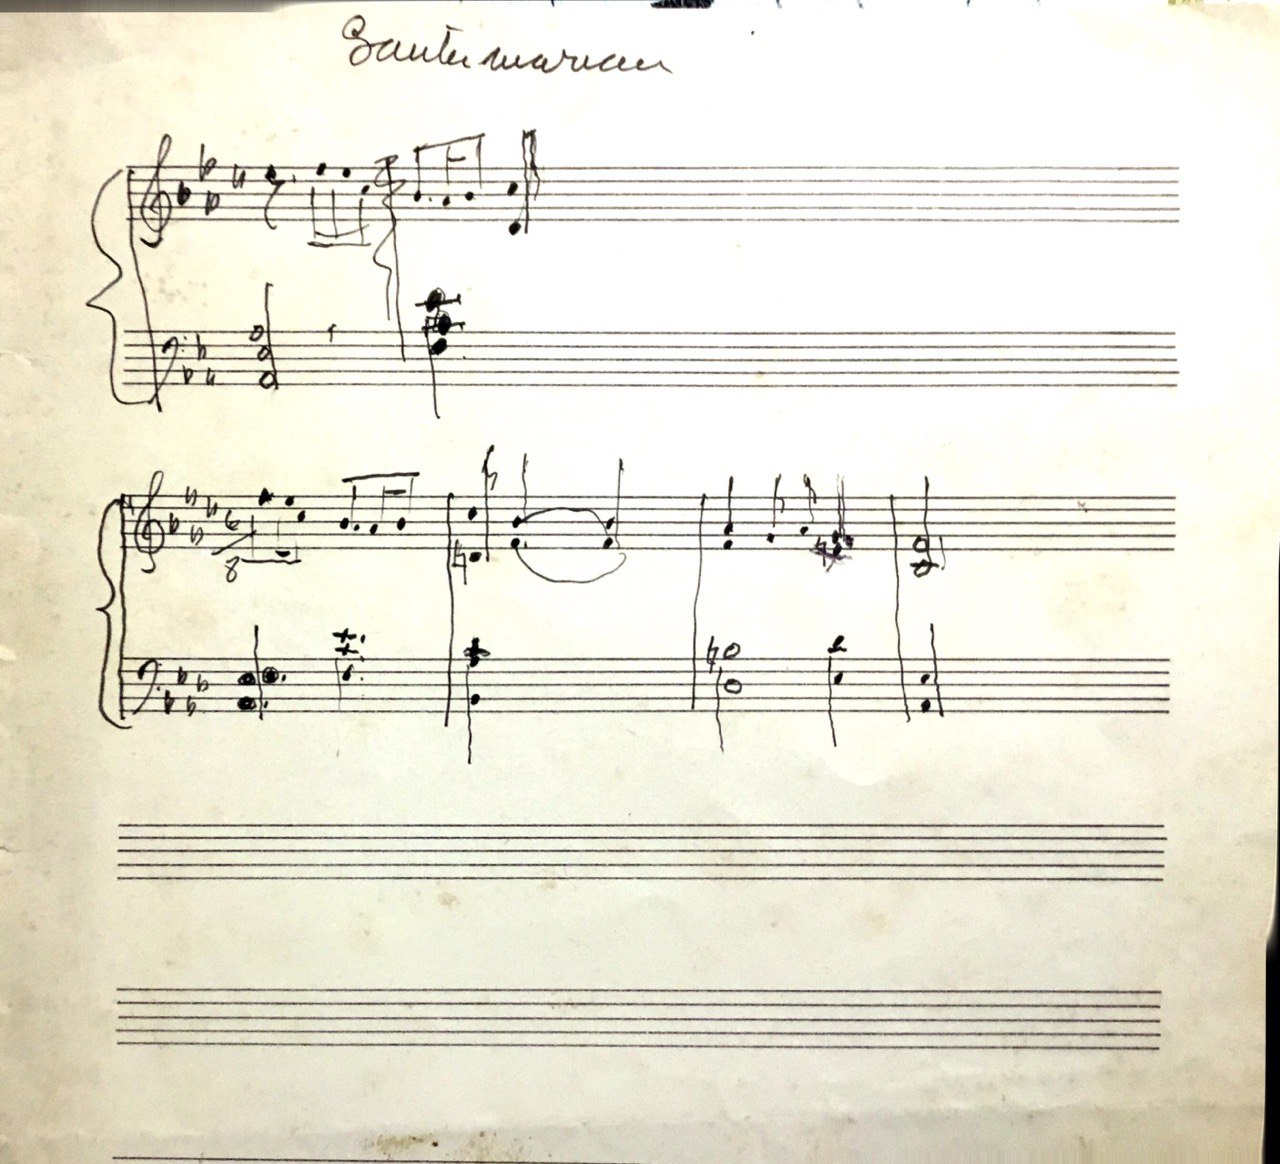
\includegraphics[width=0.6\textwidth]{img/manuscrito1}\\
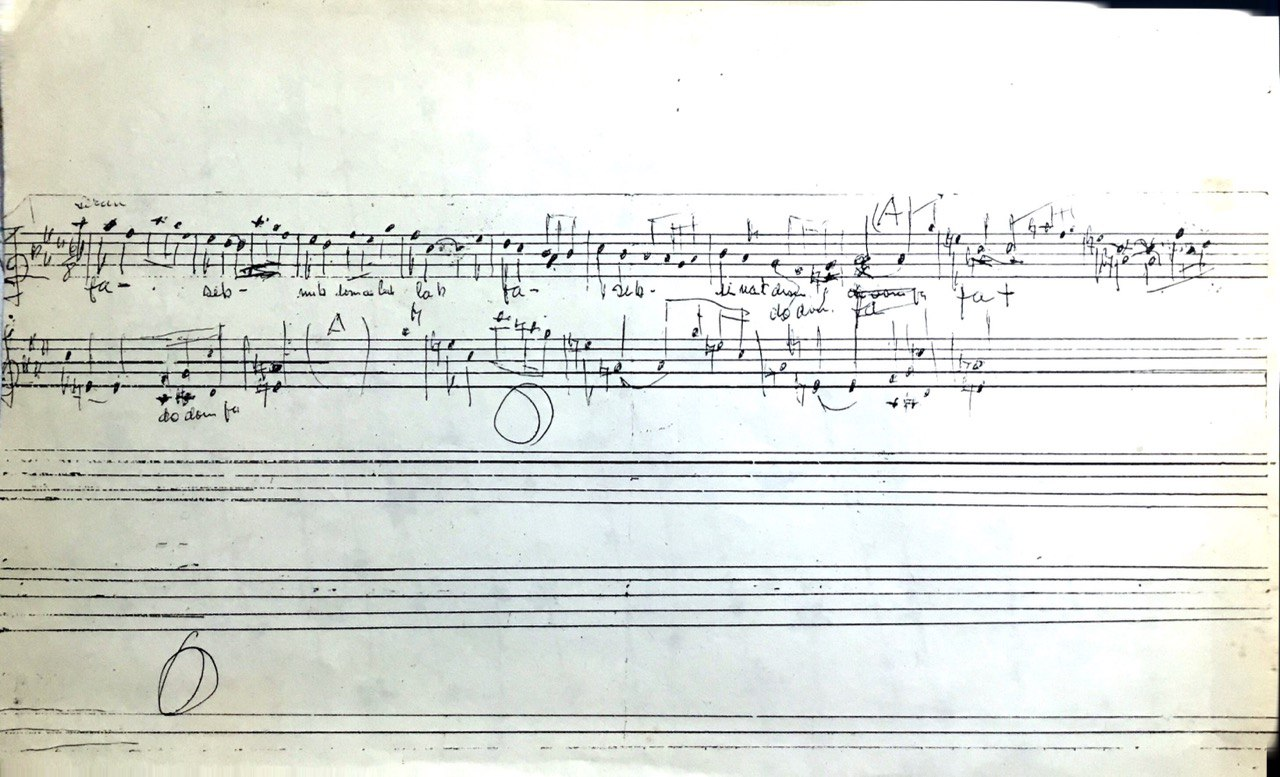
\includegraphics[width=0.6\textwidth]{img/manuscrito2}
\caption[Dos fragmentos de la caligrafía de Gustavo Leguizamón.]{Dos fragmentos\footnote{Fragmentos facilitados pon Juan Martín Leguizamón, hijo del «Cuchi».} de la caligrafía de Gustavo Leguizamón.}
\label{fig:manuscritos}
\end{minipage}
\end{figure}

Si comparamos la caligrafía de las Figuras~\ref{fig:partitura} y \ref{fig:manuscritos}, se hace evidente que es la misma mano la que trazó todos esos signos. El testimonio de \textsc{Juan Martín Leguizamón}, hijo de Gustavo, confirma que la letra sobre el primero de los fragmentos de la Figura~\ref{fig:manuscritos} es, efectivamente, la caligrafía de su padre.


\section{Notas editoriales}
\label{sec:notas-editoriales}

La partitura manuscrita de Leguizamón (ver Figura~\ref{fig:partitura}) presenta algunos errores ortográficos que, a modo de corrección editorial, modificamos en la versión digitalizada de la página~\pageref{partitura-digitalizada}. A continuación, pormenorizamos y justificamos los cambios realizados.

En la línea intermedia en los primeros compases de la introducción hay un descenso cromático \hbox{\musncp{\key f \major d''2 cis'' c'' }.} El \hbox{\nota{do\sostenidotxt}{5},} en su significado musical. no es una nota descendente sino todo lo contrario; por eso corresponde escribir \hbox{\musncp{d''2 des'' c''}.}

En el compás 8, en la mano derecha encontramos un \musncp{dis'} en un acorde \acorde.V..\bemoltxt9.7.\sostenidotxt3./II, es decir \hbox{\musncp{<d' fis' a' c'' es''>}.} Por supuesto, ese \nota{mi\bemoltxt}{4} se dirige, en el pulso siguiente, a \nota{re}{4} \hbox{\musncp{<es' fis' c''>\glissando d' },} lo que justifica doblemente el cambio de \nota{re\sostenidotxt}{4} a \nota{mi\bemoltxt}{4}. El caso se repite de manera similar en el compás 16.

En los compases 33 y 34, una voz intermedia desciende cromáticamente \musncp{\clef alto \key f \major b bes a}. Al estar distribuida dicha voz entre las manos derecha (el \nota{si\becuadrotxt}{3}) e izquierda (el \nota{si\bemoltxt}{3} de compás 33 y el \nota{la}{3} de compás 34), se hace, aunque no necesario, preferible aclarar el \musncp[voffset=4pt]{\clef bass \key f \major bes?} con la alteración sobreentendida por armadura de clave con su notación de precaución, encerrada entre paréntesis.

En el penúltimo compás, el \nota{la\bemoltxt}{4} de la mano derecha se cambió por \nota{sol\sostenidotxt}{4} por ser éste la quinta aumentada del acorde de dominante de Fa mayor, el cual se dirige ascendiendo por semitono al \nota{la}{4} del acorde final.

\newpage
\section{Himno a la Universidad Nacional de Salta}\label{partitura-digitalizada}

\begin{flushright}
Música: \textsc{Gustavo Leguizamón}\\
Letra: \textsc{Miguel Ángel Pérez}
\end{flushright}

\lilypondfile[staffsize=11]{part/leguizamon-himno_unsa.ly}

\chapter{Bitonalidad y tonalidad en la música de Leguizamón}
\label{cap:bitonalidad-tonalidad}

\begin{figure}[H]
\centering
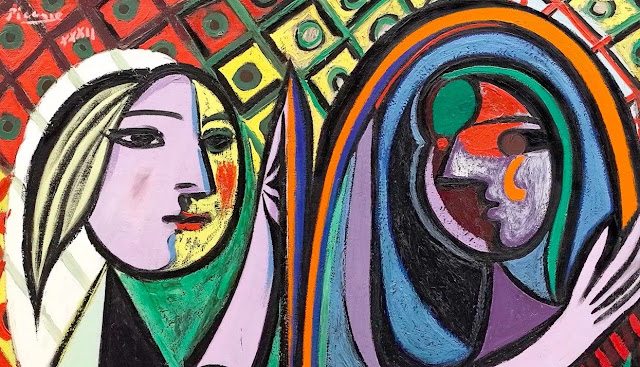
\includegraphics[width=0.8\textwidth]{img/picasso-1932}
\caption{\textsc{Pablo Picasso}. Fragmento de \emph{Joven mujer delante de un espejo}, 1932.  Óleo sobre lienzo, 162.3 x 130.2 cm. MOMA, Nueva York.}
\label{fig:picasso-1932}
\end{figure}

\section{Bitonalidad}
\label{sec:bitonalidad}

Hay una característica central en la obra musical de \textsc{Leguizamón}, indicada en alguna entrevista televisiva por el mismo autor: la presencia simultánea de dos imágenes sonoras conformando una única imagen compleja. La comparación con la pintura de \textsc{Pablo Picasso} es inevitable: una imagen compleja producto de la superposición de dos rostros, uno de frente y uno de perfil (ver Figura~\ref{fig:picasso-1932}).

Los acordes triadas fueron, durante mucho tiempo, la fundamentación del pensamiento armónico en la música occidental. Avanzado el siglo XIX, la creciente tendencia a utilizar acordes de más de tres notas no dejaba de hacer referencia a una única fundamental de cada uno de dichos acordes. Los llamados acordes \emph{errantes}\footnote{Un acorde errante ---tal es la denominación de \textsc{Arnold Schoenberg}--- es un acorde que es capaz de cumplir la misma función tonal en más de una tonalidad no-homónima. Típicos ejemplos de ellos son los acordes de séptima disminuida, los de quinta aumentada, los de sexta aumentada y los séptima dominante a distancia de semitono ascendente respecto a la tónica.}, aunque en sí poseen una única fundamental, sí pueden estar respondiendo a más de una tónica, por lo que su aparición en la escena musical es un importante antecedente para el surgimiento de la música politonal, es decir la música que tiene más de una tónica al mismo tiempo.

Otro antecedente histórico presente en la tonalidad que ayudó a desembocar en la bitonalidad está presente ya en el modo menor, cuando se enlaza el III grado con el \acorde.V..\sostenidotxt3..., enlace en el que la quinta del tercer grado ---en La menor, \emph{sol}--- se relaciona con la tercera del \acorde.V..\sostenidotxt3... ---\emph{sol\sostenidotxt}. La normativa tonal, justamente para evitar la presencia de dos tónicas simultáneas, prohíbe lo que se conoce como \emph{falsa relación}, obligando a introducir la tercera del \acorde.V..\sostenidotxt3... en la misma voz que la quinta del III grado produciendo así un ascenso cromático de la voz que impide la interpretación perceptual de la presencia de más de una tónica simultánea. Sin embargo, muy habitualmente en las prácticas populares la norma no se observa, apareciendo de facto la bitonalidad. El modo dórico, tan presente en algunas manifestaciones musicales folclóricas de Sudamérica que nutrieron al universo musical de Leguizamón, tiene en potencia la posibilidad de la bitonalidad, especialmente en la relación entre los grados VI y \acorde.IV..\sostenidotxt3..., donde la fundamental del primero y la tercera del segundo, de sucederse en voces diferentes, o de estar ésta en la línea melódica mientras el acompañamiento transcurre sobre el VI grado\footnote{Este fenómeno puede encontrarse en grupos folclóricos como \emph{Los Fronterizos}.}, la manifestación de la bitonalidad es ya un hecho.

\textsc{Ravel}, \textsc{Bartók} y \textsc{Stravinsky} son algunos de los exponentes europeos que explicitan en su obra la presencia de más de una tónica en la simultaneidad. \textsc{Villalobos}, \textsc{Revueltas} y \textsc{Ginastera} también lo hacen en América. \textsc{Leguizamón}, \textsc{Piazzolla} y \textsc{García}, más acá en el tiempo, incluyen en sus composiciones estas técnicas que ofrecen a los oyentes una complejidad armónica abordable por los oídos contemporáneos. Las resistencias y oposiciones que enfrentaron todos los compositores anteriormente citados, hoy ya han sido superadas, hoy ya encuentran en las percepciones de las mayorías eco favorable para esas sonoridades que fueran novedad durante el siglo pasado.

\section{Tonalidad y arquetipos}
\label{sec:tonalidad-arquetipos}

Dos son los arquetipos musicales rastreables en prácticamente todas las culturas humanas: la escala y el arpegio. Éste surge del despliegue en el tiempo de los cuatro primeros parciales de un sonido armónico\footnote{Un \emph{sonido armónico} es el que es susceptible de ser cantado, un sonido con altura determinada, un sonido que en su estructura de frecuencias conformantes existe una relación de múltiplos enteros de la frecuencia fundamental.}, mientras que aquélla es, en sus versiones ascendente y descendente, la garantía de un camino perceptualmente transitable a la vez que tranquilizante. Tanto una escala como un arpegio son fáciles de cantar para la inmensa mayoría de seres humanos, y si es fácil de cantar es porque es fácil de percibir.

\label{par:puente}Un \emph{puente de segundas}, en composición de melodías, es «esconder» una escala dentro de una melodía más compleja para que el oyente o el cantante tengan disponible ese arquetipo para su tranquilidad y facilidad de ejecución. Raro es el himno ---especialmente himnos nacionales--- que no posea en su línea melódica un puente de segundas. Podemos poner como ejemplo el himno ruso:

\begin{figure}[H]
\begin{ly}[ragged-right]
\relative {
  \key f \major
  \time 4/4
  \slurDashed
  a''2 ( g8 f e f
  g2 ) ( c,
  f ) ( e8 d c d
  e2 ) ( a,
  d4 ) ( c8. bes16 c4. ) f,8
  f'4 e8. d16 c2
}
\end{ly}
\caption{Puente de segundas en los himnos del mundo: himno de Rusia.}
\label{fig:himno-ruso}
\end{figure}

Marcado con ligaduras punteadas, en la Figura~\ref{fig:himno-ruso} podemos observar el puente de segundas presente en el estribillo del himno de Rusia, conformando una escala descendente \musncp{\relative {a''2 g f e d c}} que dota a esta línea melódica tanto de belleza como de facilidad de entonación para muchas personas.

\begin{figure}[H]
\begin{ly}
\relative {
  \key f \major
  \time 2/4
  \partial 8
  c'8
  \slurDashed
  f4. ( f8
  f d e f
  g4 ) ( g8 f
  e4. c8
  a'4. ) ( a8
  a f g a
  bes4 ) bes8 a
  g4.
}
\end{ly}
\caption{Puente de segundas ascendentes en el himno de Leguizamón.}
\label{fig:segundas-ascendentes-himno}
\end{figure}

Observando esta característica de la tradición hímnica, Leguizamón construye la línea melódica del Himno a la Universidad Nacional de Salta sobre un puente de segundas ascendentes \musncp{\relative {\key f \major f'2 g a bes}} en la primera parte (ver Figura~\ref{fig:segundas-ascendentes-himno}) y otros dos puentes de segundas descendentes \musncp{\relative{\key f \major f''2 ( e d c\glissando ) a ( g f )}} en la segunda parte. El hecho de poseer dos puentes de segundas, donde el primero empieza en \nota{fa}{5} y termina en \nota{do}{5}, y el segundo empieza y termina en \nota{la}{4} y \nota{fa}{4}, muestra al oyente y al intérprete ---en forma aún más sutil que la escala--- el arpegio de Fa mayor \hbox{\musncp{f''2 c'' a' f'},} representante melódico él de la tónica. Así, los dos arquetipos musicales presentes en toda cultura humana, presentes también están en la melodía del Himno a la UNSa de Leguizamón.

\begin{figure}[H]
\centering
\begin{ly}
\relative {
  \key f \major
  \time 2/4
  \partial 8
  c''8
  \slurDashed
  f4. ( f8
  f d e f
  \slurHalfDashed
  e4 ) ( c8 a
  c4. )
}
\end{ly}
\begin{ly}
\relative {
  \key f \major
  \time 2/4
  \partial 8
  \slurHalfDashed d''8 (
  bes4 ) bes
  bes4.
}
\end{ly}
\begin{ly}
\relative {
  \key f \major
  \time 2/4
  \partial 8
  \slurHalfDashed
  c''8 (
  a ) \slurDashed ( g a f
  g ) ( d e c
  f4. )
}
\end{ly}

\vspace{0.5cm}

\begin{ly}[notime]
\layout {
  \context {
    \Voice
    \consists Horizontal_bracket_engraver
  }
}
\relative {
  \key f \major
  <<{f''2\startGroup e d c\stopGroup s s} \\ {s2 s bes\startGroup a g f\stopGroup}>>
}
\end{ly}
\caption{Arpegio y escala en la melodía.}
\label{fig:arpegio-escala-cuchi}
\end{figure}

\noindent En rigor de verdad, \musncp{\relative{\key f \major f''2 ( e d c\glissando ) a ( g f )}} no es una fiel representación de la estructura melódica de los compases 26 al 34, sino el último Fragmento presentado en la Figura~\ref{fig:arpegio-escala-cuchi}, donde se puede ver una especie de solapamiento del desarrollo de dos puentes de segundas, uno desplegando el tetracordio superior \nota{fa}{5}-\nota{do}{5}, y otro cerrando el ciclo de la octava con el tetracordio inferior \nota{si\bemoltxt}{4}-\nota{fa}{4} de la tonalidad de la pieza. Ese solapamiento entre tetracordios se produce en los compases 30 y 31, visible en el segundo fragmento de la Figura~\ref{fig:arpegio-escala-cuchi}, compases éstos que presentan el verso \emph{hasta que al fin}, verso que rompe con la precedente simetría de 11 sílabas mostrado en el Cuadro~\ref{tab:ritmo-letra}. Aunque por un lado el solapamiento oscurece la presencia del arpegio, por otro ---y a pesar de estar en parte débil de tiempo--- el \nota{do}{5} en el \emph{levare} del compás 32 pasa a tener, en la percepción del oyente, un lugar jerarquizado por ser el inicio de un envión final que nos deposita en el último tramo de la pieza, y al ser esta nota perceptualmente importante, garantiza y aclara la presencia de la estructura arpegiada, la cual también está afianzada por la presencia del \nota{do}{5} del compás 29, en tiempo fuerte y con una duración de una \negrap\ que cierra la palabra \emph{ofrendarán}.

Aún no hemos llegado a la certeza estructural, ya que en la primera parte del descenso (compases 26 al 29, ver Figura~\ref{fig:arpegio-escala-cuchi}, primer fragmento) observamos una estructura \hbox{\musncp{\key f \major f''2 e'' c''},} no \musncp{\key f \major f''2 e'' d'' c''}, donde el \nota{re}{5} mencionado como estructural aparece en forma diferida y asociada a la relación de tercera descendente en los compases 30 y 31 con \emph{levare} transcripto en el segundo fragmento de la Figura~\ref{fig:arpegio-escala-cuchi}, y que completa juego con el tercer fragmento de la misma Figura con el descenso de tercera \musncp{c''2 a'}, conformando entre las tres partes una sucesión de terceras \musncp{\key f \major <e'' c''>2 <d'' bes'> <c'' a'>}, presentada parcialmente en el cuarto fragmento de la citada Figura, de carácter analítico, como solapamiento entre tetracordios. El no haber dicho en primer término lo de la sucesión de terceras y sí haber mencionado lo de la sucesión de tetracordios tiene que ver con que esta sucesión es estructuralmente más importante que la sucesión de terceras debido a que a partir del \emph{levare} del compás 34 hasta el final nos encontramos con una melodía cuya estructura responde, una vez más, a una demarcación de los inicios y finales de los tetracordios de la escala de Fa mayor \hbox{\musncp{\key f \major f'2 bes' c'' f''},} tal como muestra la Figura~\ref{fig:final-melo-estructura}.

\begin{figure}[H]
\begin{ly}
\relative {
  \key f \major
  \time 2/4
  \partial 8
  c'8
  \slurDashed
  f4. ( f8
  f d e f
  bes4. ) ( bes8
  bes g a bes
  c4 ) ( f8 g
  d4 e
  f2 ) \bar "|."
}
\end{ly}
\caption{Final de la melodía: estructura tetracordal.}
\label{fig:final-melo-estructura}
\end{figure}


La estructura melódica completa queda, pues, definida principalmente por notas que delimitan al tetracordio inferior puestas en forma ascendente y conectadas por un puente de segundas, seguidas por notas que delimitan el tetracordio superior conectadas por un \nota{mi}{5}, seguido por nuevamente el tetracordio inferior esta vez presentado en forma descendente como puente de segundas, para finalmente representar otra vez el tetracordio inferior, esta vez en un ascenso final y por salto directo entre el \grado{1} y \grado{4} grados (\emph{fa-si\bemoltxt}), finalizando con el tetracordio superior (\emph{do-fa}) haciendo oír sus notas extremas primero en forma directa (salto) y luego recorriendo el resto del tetracordio (\emph{re-mi-fa}).

\begin{figure}[H]
\begin{ly}[notime]
\layout {
  \context {
    \Voice
    \consists Horizontal_bracket_engraver
  }
}
\relative {
  \key f \major
  \hide Stem
  \slurHalfDashed
  f'2^"c.18"\startGroup g a bes\stopGroup \bar "||"
  f'^"c.26"\startGroup e4 ( c2\stopGroup ) \bar "||"
  d4^"c.30" ( bes2\startGroup ) c4 ( a2 ) g f\stopGroup ~\bar "||"
  f2^"c.34"\startGroup bes\stopGroup
  \slurHalfSolid
  c^"c.38"\startGroup ( f4 ) d2 e f\stopGroup \bar "|."
}
\end{ly}
\caption{Estructura de la melodía.}
\label{fig:estructura-melodia}
\end{figure}

Además de haber hecho presente los arquetipos de escala y arpegio, como acabamos de ver, hace el autor aparecer un tercer arquetipo: el de dividir la octava en dos partes iguales, dos cuartas justas conteniendo cada una de ellas cuatro sonidos, es decir un \emph{tetracordio}. Innumerables y de diversas culturas son los ejemplos ancestrales de uso de estructuración de melodías en esta forma, usando como puntos de apoyo de las frases musicales a las notas de partida y llegada de cada uno de los tetracordios en los que se secciona la octava, base de toda música tonal. Desde cantos antifonales y responsoriales donde grupos antagónicos o complementario, o un líder y sus seguidores cantan alternativamente unos en las notas de un tetracordio y los otros responden sobre las notas del otro tetracordio. Esa genética cultural, además de los dos arquetipos universales, es la que se encuentra inscripta en la melodía del Himno a la Universidad de Salta de Gustavo Leguizamón.


\section{Tonalidad de tonalidades}
\label{sec:tonalidad-tonalidades}

Desde el alto barroco hay conciencia en los compositores acerca de una tonalidad que contiene a otras tonalidades. El sistema tonal es la síntesis de los doce modos eclesiásticos\footnote{La teoría musical de la Edad Media definió un total de siete modos, \emph{dórico, frigio, lidio, mixolidio, eólico, jónico y locrio}, a los que denominó \emph{modos auténticos}, y derivó de ellos siete más, los llamados \emph{modos plagales}. De esos catorce modos eliminó dos (locrio e hipolocrio) por considerarlos no aptos para la práctica musical vigente entonces.} resumidos en los modos mayor y menor. Al ser siete los grados armónicos (acordes) de una tonalidad, donde tres son mayores, tres menores y uno disminuido, se observó y no se desaprovechó la oportunidad de interpretar a cada grado mayor o menor como una tonalidad entera dentro de la tonalidad. Cada una de estas seis tonalidades con sus propios grados armónicos. El VII grado del modo mayor ---y el II del modo menor--- sufrió, en este sentido, el mismo destino que en su momento sufriera ---y por motivos similares--- el modo locrio: la ignorancia, la periferia desde la cual luego montaría éste su revolución\footnote{El VII grado del modo mayor y el II del modo menor contienen el intervalo más complejo de percibir, el \emph{tritono}, el cual desempeñó y desempeña un papel central en el desarrollo de la composición musical}. Al ser la tonalidad un sistema jerarquizado, donde cada nota cumple función y cada conjunto estandarizado de notas (acordes) cumple función en un escenario donde se libra una lucha por el poder, por el privilegiado lugar de la tónica, a la vez los grados armónicos subordinados a cada grado de la tonalidad cumplirán, en el contexto general, la misma función que su «jefe regional», su grado continente cumple en la tonalidad principal. Por ejemplo, aunque un II grado, en general, cumple una función de \emph{subdominante}, el II grado de un V grado (II/V) cumple, en la tonalidad principal, la función que cumple el V grado, es decir función de \emph{dominante}, o, dicho de otra manera, «donde manda capitán V no manda marinero II/V».

Esta noción de \emph{metatonalidad}, de tonalidad de tonalidades, en la práctica musical folclórica argentina se ve acotada casi exclusivamente a la presencia de \emph{dominantes secundarias}, es decir a utilizar el V grado de cada grado mayor o menor de la escala. Usar otro grado que no sea el V/x es, en la música popular argentina de medio siglo atrás un inequívoco síntoma de arte evolucionado y con un grado de complejidad a la que afortunadamente la sociedad argentina está acostumbrada por poseer una notable riqueza en sus músicas de consumo masivo. Volvemos acá a mencionar a Piazzolla, podemos agregar a Mariano Mores, y saludar nuevamente a Charly García como pares de Leguizamón en cuanto compositores que presentan a su público una elaboración armónica que no lo subestima.

El compás 16 del \emph{Himno} ya nos presenta un acorde \hbox{\musncp[voffset=-4pt]{\key f \major \clef alto <d c' es' fis' a' c''>2},} ajeno éste al diatonimso de Fa mayor. Por ello, para hallar el significado armónico de tal acorde nos conviene bucear en alguna de las regiones, en algunos de los grados de Fa mayor. En este caso, notamos que la estructura del acorde corresponde a una dominante, pero dominante de qué grado es la pregunta que debemos hacernos, V grado de qué grado, y al ser \emph{re} la fundamental de dicho acorde, sale a la luz que es V/II, es decir dominante de la relativa menor de la subdominante (D/rS, SOLm), con novena y séptima menores, por lo que su cifrado es \acorde.V..\bemoltxt9.7.\sostenidotxt3./II. Hasta acá, nada fuera de libreto respecto a los usos habituales en la música popular. Sin embargo, lo notorio surge de inmediato al resolverse este acorde no donde se espera, es decir en el II grado de Fa, sino ¡sobre el V grado de la tonalidad principal! Es muy habitual, en una música que renuncia a lo revolucionario en favor de la transformación ---y la de Leguizamón lo es--- proceder modificando el camino que pasa por tres puntos \emph{a, b, c} a un camino que da por obvio al punto \emph{b} pasando directamente de \emph{a} a \emph{c}. Así, cuando se espera la semicadencia V/II - II - V al final de la introducción del \emph{Himno}, nos encontramos con el enlace directo V/II - V, del punto \emph{a} al punto \emph{c} sin escala intermedia. Suena novedoso, pero no revolucionario; transforma, innova al tiempo que no deja a los oyentes en un terreno ni hostil ni completamente desconocido, a la vez que no desprovisto de sorpresa.

El mismo acorde es oído con anterioridad, en el compás 8, también en la introducción de la pieza, pero en esta ocasión el acorde no se dirige hacia la dominante, sino que cumple la función formal de suspender la semifrase antes de retomar la segunda semifrase, la cual parte de tónica. Si el camino \emph{a - b - c}, es resumido en \emph{a - c} en los compases 16 y 17, en los compases 8 y 9 se resume a la presencia del único punto inicial del camino, el punto \emph{a}, el acorde \acorde.V..\bemoltxt9.7.\sostenidotxt3./II, sin resolución alguna, suspendiendo, dejando abierta la semifrase inicial de la introducción del himno.

Tanto en su aparición en compás 8 como en la de compás 16, el V/II está presente bajo el fragmento melódico \mus{\key f \major \time 2/4 c''4 ~ \tuplet 3/2 {c''8 a' bes'} c''4_"V/II"}. La diferencia formal y consecuentemente funcional está dada por el nada irrelevante hecho de la repetición del fragmento melódico en compás 16 con \emph{levare}, siendo \mus{\key f \major \time 2/4 \partial 4 \tuplet 3/2 {r8 a' bes'} c''4_"V/II" ~ \tuplet 3/2 {c''8 a' bes'} c''4_"V"} una semicadencia sobre el V grado que convierte al V/II en un acorde con función subdominante que precede justamente al V, mientras que en compás 8, al no estar repetido el motivo melódico, el mismo acorde V/II cumple sorpresivamente la función de \emph{dominante}, ya que la ausencia del V con posterioridad al V/II, lo hace indirectamente representante de la dominante, aunque tal acorde surja de la región de la relativa de la subdominante. Aunque sólo esté presente el marinero, el que sigue mandando es el capitán.

\section{Funciones armónicas y bitonalidad}
\label{sec:funciones-bitonalidad}

Para finalizar este breve análisis del \emph{Himno} en sus aspectos armónicos sobresalientes, ponemos el foco en los compases del 27 al 29:

\begin{figure}[H]
\centering
\begin{ly}
manoderecha = \relative {
  \clef treble
  \key f \major
  \time 2/4
  \set Score.currentBarNumber = #27
  \bar ""
  <b' f'>8 d <b e> f'
  <f, e'>4 <g c>8 <e a>
  <es fis c'>4. d'8

}
manoizquierda = \relative {
  \clef bass
  \key f \major
  \time 2/4
  b,8 gis' d'4
  <f,, c' a'>2
  <d' c'>
}

\score {
  \new PianoStaff <<
    \new Staff \manoderecha
    \new Staff \manoizquierda
  >>
}
\end{ly}
\caption{¿Dominante del III grado resolviendo en I?}
\label{fig:V-III}
\end{figure}

El acorde que encontramos en el compás 27 es el \acorde.V.\becuadrotxt5.9.7.\sostenidotxt3./III, acorde que convencionalmente resuelve sobre su «jefe» regional, el III grado. Sin embargo, en compás 28, en lugar de ese esperado III nos topamos de frente con el \acorde.I..9.7.., el cual, en compás 29, resuelve sobre el ya mencionado, en sección~\ref{sec:tonalidad-tonalidades}, \acorde.V..\bemoltxt9.7.\sostenidotxt3./II, cumpliendo él, una vez más, la función de semicadencia ---esta vez dejando abierta la expectativa de resolución sobre el II grado que, esta vez, sí se cumple en compás 30, inicio de una nueva frase y un nuevo verso. ¿Cómo se explica que el \acorde.V.\becuadrotxt5.9.7.\sostenidotxt3./III resuelva en \acorde.I..9.7..? Si observamos, en la Figura~\ref{fig:V-III}, la mano derecha del compás 28, notaremos que la sensible descendente \nota{fa}{5} del compás anterior presente en la melodía resuelve sobre el \nota{mi}{5}, séptima del I grado, siguiendo la línea melódica con el despliegue del arpegio de La menor, apoyado por el \emph{voicing} que presenta, bajo el \emph{do} a la novena del I y bajo el \emph{la} la séptima del mismo grado, pero que a la vez son la séptima y la quinta del acorde de La menor. ¿Estamos ante una «pincelada» de bitonalidad, donde conviven los centros tonales de \emph{fa} y \emph{la}? Nuestra respuesta: sí. El \acorde.V.\becuadrotxt5.9.7.\sostenidotxt3./III sí está resolviendo sobre un \acorde.III.6.7..., que al tener en el bajo el \nota{fa}{2} (mano izquierda) produce un acorde complejo que, sin profundizar, tendemos a reconocer como un acorde \acorde.FA..9.7.. y no como un \acorde.LAm.Fa.7.... En definitiva, en este pasaje del \emph{Himno}, como en tantos otros pasajes toda de la obra musical de Leguizamón, tenemos, al mismo tiempo, un rostro de frente (\emph{fa}) y de otro perfil(\emph{la}), como si de una pintura de Picasso se tratara.

\chapter{Caminos posibles}
\label{cap:caminos}

Hay una buena noticia: una pieza del «Cuchi» Leguizamón ha sido rescatada. Para que ella pueda ser considerada el Himno de la Universidad Nacional de Salta hay que recorrer alguno de posibles caminos para allanar las dificultades que la pieza, por algunas características que posee, impone.

\section{Tonalidad y registro}
\label{sec:tonalidad-registro}

Entre esas características está, en primer lugar, la tesitura de la voz humana para la que fue escrita, que no condice con el registro de la media de la población de Salta (ni la mundial). Adaptar la pieza transportándola un tono y medio abajo, a la tonalidad de Re mayor ---recomendable para orquesta---, o dos tonos abajo, a la tonalidad de Re\bemoltxt\ mayor ---recomendable para banda de vientos--- es imprescindible para que la línea melódica no quede accesible solamente a voces naturalmente dotadas o educadas musical y técnicamente. Sin embargo, el transporte no es gratis: lo que en Fa mayor es tocable en el piano, tanto en Re como en Re\bemoltxt\ mayor cobra dificultades, especialmente en los intervalos de décima, ya que no es lo mismo tocar el intervalo \musncp[voffset=-1pt]{\key f \major \clef bass <f, a>} que tocar el intervalo \hbox{\musncp[voffset=-2pt]{\key d \major \clef bass <d, fis>},} el cual requiere de una mano más grande. Lo mismo sucede con el transporte a Re\bemoltxt\ mayor. De todos modos, estos transportes, lo recordemos, están siendo sugeridos para versiones orquestadas o arregladas para banda militar u orquesta sinfónica. Claro está que no deja de ser un dilema tener, o no, versiones de un himno en diferentes tonalidades. No recomendamos acá la diversidad. Debe elegirse una, y adaptar las cuestiones técnicas a las diversas y posibles instrumentaciones. Esto favorecerá la el aprendizaje y la memoria colectiva de la melodía.

\subsection{Versión transportada a Re mayor}
\label{subsec:transporte-re}

\lilypondfile[staffsize=11]{part/leguizamon-himno_unsa-re.ly}

\subsection[Versión transportada a Re\bemoltxt\ mayor]{Versión transportada a Re\bemol\ mayor}
\label{subsec:transporte-reb}

\lilypondfile[staffsize=11]{part/leguizamon-himno_unsa-reb.ly}


\subsection{Tonalidad recomendada}
\label{subsec:tonalidad-recomendada}

Como Re\bemoltxt\ tiene sus bemoles, \emph{Re mayor}, aunque no sea la más facilitadora para bandas de vientos ---como lo son las bandas militares---, es mi recomendación, ya que sí facilita el canto para una mayoría de personas perteneciente a nuestra sociedad, la salteña, donde por razones de conformación étnica encontramos un amplio segmento de voces femeninas clasificadas en la voz de \emph{mezzasoprano}\footnote{Una voz ni muy aguda ni muy grave.}, y lo propio en las voces masculinas inscriptas en el registro de \emph{barítono}\footnote{Al igual que las \emph{mezzosopranos} en las voces femeninas, los \emph{barítonos} poseen facilidad para sonidos intermedios, ni muy agudos como los de un \emph{tenor}, ni muy graves como los de un \emph{bajo}.}. A la vez, también Re mayor facilita la ejecución en instrumentos de cuerda frotada\footnote{Violines, violas, violoncellos, contrabajos.}, instrumentos que cuando se entiende a la orquesta sinfónica desde una óptica clásica conforman la base de dicho organismo musical, y a la vez son capaces de organizarse en agrupaciones de cámara como tríos (violín, viola, violoncello), cuartetos ( dos violines, viola, cello) o quinteto (cuarteto más contrabajo), agrupaciones éstas que pueden contratarse con mucho menos presupuesto y con más ofertas que una orquesta si se desea tener un evento en vivo donde presentar el \emph{Himno}, himno que por su carácter íntimo \emph{pide} ser interpretado con instrumentos que sin esfuerzo expresen ese carácter, como los son los instrumentos de cuerdas ---y no tanto los instrumentos de bronce, aunque con buenos intérpretes siempre todo es posible.

La versión para piano y voz, si se elige Re mayor como única tonalidad para todas las versiones del \emph{Himno} ---criterio éste que ejercería una labor docente en la enseñanza-aprendizaje de la melodía en la población sin instrucción musical---, debe ser adaptada en parte para subsanar los ya mencionados problemas de tocabilidad surgidos del transporte, siendo necesaria la adaptación de algunos intervalos para que la mano humana acceda a ejecutar sobre un teclado esta pieza. Por otro lado, no parece negociable la existencia de una versión para voz y pianos, siendo esta formación la original en la composición de Leguizamón y la que mejor expresa el carácter íntimo de la canción.


\section{Orquestación, o arreglo}
\label{sec:orquestacion-arreglo}

\emph{Orquestar} una pieza musical consiste en respetar tanto las notas como la textura de un original y presentarlo en una versión que viste a esa pieza original con los timbres de los instrumentos de una orquesta. Así, por ejemplo, si se orquesta el \emph{Himno a la Universidad Nacional de Salta}, composición original para canto y piano, la orquesta \emph{debe} re-presentar al piano de forma totalmente fiel en cuanto a notas se refiere, repartiendo los sonidos simultáneos entre los instrumentos de la orquesta que el orquestador decida utilizar en cada momento de la pieza.

\emph{Arreglar para orquesta} una música determinada implica más que una orquestación, ya que lo que se busca es una \emph{versión} de la composición original con pinceladas de composición orientadas a nutrir a la composición original de elementos compatibles con el lenguaje propio de la música sinfónica (si se trata de una orquesta sinfónica), o de cámara (si se trata de una agrupación de pocos instrumentos). Un arreglo, dependiendo de las decisiones artísticas del arreglador, puede orientarse hacia una versión completamente alejada del espíritu de la música original en un extremo, o hacia el máximo respeto por sostener dicho espíritu en la versión en el otro extremo. En el medio, por supuesto, de todo hay.

Al ser el \emph{Himno} una pieza de muy corta duración, aunque se decida ---y es necesario que así sea--- un \emph{ritornello} que repita toda la pieza para permitir el doble de letra de lo que el poema de Pérez posee, se necesita tanto la composición de un par de compases que encause el retorno al inicio (primera y segunda casilla en la escritura de la partitura) como, quizás, una ampliación de la introducción que será, al repetirse, también \emph{intermezzo}. Esto, evidentemente, no es orquestar, por lo que esta es nuestra recomendación: \emph{arreglar el \emph{Himno}, tanto para piano y voz como para orquesta sinfónica y conjuntos de cámara como cuarteto de cuerdas, por ejemplo.}

Condición \emph{sine qua non} para acometer cualquier arreglo es, antes que nada, tener definida una letra que dé marco semántico al arreglador para que éste pueda representarlo musicalmente en su trabajo.


\backmatter
\begin{appendices}
\chapter{Código fuente de la partitura}
\label{cap:codigo}

Para la edición de la partitura hemos utilizado \texttt{GNU/LilyPond}\footnote{\texttt{\textbf{GNU/LilyPond}} es software libre, descargable desde \url{www.lilypond.org}. Está disponible para los sistemas operativos más importantes. \texttt{\textbf{Hacklily}}, \url{https://www.hacklily.org/} es una implementación web de LilyPond que permite utilizar este editor de partituras en cualquier dispositivo con un navegador web y una conexión a internet. Copiando y pegando el código acá facilitado se obtiene un archivo PDF de la partitura del Himno a la UNSa de Leguizamón y Pérez.}. El código para compilarla, a continuación.

\begin{lstlisting}[
  % numbers=left,
  % numberstyle=\tiny,
  language=tex,
  backgroundcolor=\color{yellow!10},
  breaklines=true,
]
\version "2.24.1"

global = {
  \key f \major
  \time 2/4
  \tempo "Introducción" 4 = 60
  \partial 4 s4
  s2*16
  s4.
  \tempo "Canto" s8
  \bar "||"
  s2*23
  \bar "|."
}

melodia = \relative {
  r4
  R2*16
  r4. c'8
  f4. f8
  f d e f
  g4 g8 f
  e4. c8
  a'4. a8
  a f g a
  bes4 bes8 a
  g4. c8
  f4. f8
  f d e f
  e4 c8 a
  c4. d8
  bes4 bes
  bes4. c8
  a g a f
  g d e c
  f4. f8
  f d e f
  bes4. bes8
  bes g a bes
  c4 f8 g
  d4 e
  f2
}

manoderecha = \relative {
  \tuplet 3/2 {c'''8 a g}
  \acciaccatura gis8 a d,4.
  \acciaccatura gis8 a des,4.
  \acciaccatura fis8 g c,4.
  e,16 f a c \tuplet 3/2 {g'8 f e}
  g bes,4.
  \tuplet 3/2 {<e, a>8 bes' c} \tuplet 3/2 {<f, bes d> f' e}
  <d, a' c>4 ~ \tuplet 3/2 {<d a' c>8 a' bes}
  <es, fis c'>4 \tuplet 3/2 {c''8 a g}
  \acciaccatura gis8 a d,4.
  \acciaccatura gis8 a des,4.
  \acciaccatura fis8 g c,4.
  e,16 f a c \tuplet 3/2 {g'8 f e}
  g bes,4.
  \tuplet 3/2 {<e, a>8 bes' c} <f, bes d> a'
  <f, c' f>4 ~ \tuplet 3/2 {<f c' f>8 a bes}
  <es, fis c'>4 ~ \tuplet 3/2 {<es fis c'>8 a bes}
  <e, a c>4. c8
  f4. f8
  f d e f
  <b, g'>4 <b g'>8 f'
  e4. c8
  <e a>4. <e a>8
  <e a> <c f> <e g> a
  <f bes>4 <f bes>8 a
  <e g>4. c'8
  <f, d' f>4. q8
  <b f'> d <b e> f'
  <f, e'>4 <g c>8 <e a>
  <es fis a c>4. d'8
  <f, bes>4 q
  bes4. c8
  <e, a>8 g <e a> f
  <b, g'> d e c
  f4. f8
  f8 d e f
  <f bes>4. q8
  q g <e a> bes'
  <e, a c>4 <c' f>8 g'
  <f, b d>4 <e gis e'>
  <f a c f>2
}

manoizquierda = \relative {
  \clef bass
  r4
  <g,,g'>4 <d''' f bes>
  <c, bes' e> <c' bes'>
  <f,, c' a'> <d'' a'>
  <d, a' c> <d c' f>
  <g, d'bes'> d''
  <c, bes' d> <g' d'>
  <f, c' a'> d'
  <d a' c> d'
  <g,,, g'> <d''' f bes>
  <c, bes' e> <c' bes'>
  <f,, c' a'> <d'' a'>
  <d, a' c> <d c' f>
  <g, d'bes'> d''
  <c, bes' d> <g' d'>8 <c, bes' e>
  <f, d' a'>4 d''
  <d, c'> d'
  <c, bes' d>2
  f,8 c' a'4
  <d, a' c>2
  <g, f'>4 g'
  c,8 bes' d4
  f,,8 c' d e
  f a ~ a4
  <g d'>8 cis <g d'> cis
  <c, bes' d>4 c'
  d,,8 a' f' c'
  b, gis' d'4
  <f,, c' a'>2
  <d' c'>
  <g d'>8 cis <g d'> cis
  <c, c'!>4 d'
  <f,, c' a'> <d' a' c>
  <g, f'> <c bes'?>
  f,8 c' a'4
  <d, a' c>2
  <g d'>4 cis
  <c, bes' d> c'
  <f,, c' a'> <d' a' f'>
  <g, d' b'> <c bes' d>
  <f c' d>2
}

versos = \lyricmode {
  Es -- toy so -- bre mi tie -- rra
  pa -- ra be -- ber
  el ai -- re que me~a -- lien -- ta
  y~e -- se li -- cor
  que los an -- ti -- guos dio -- ses
  o -- fren -- da -- rán
  has -- ta que~al fin,
  des -- nu -- da~el al -- ma~en -- su~es -- plen -- dor,
  re -- tor -- ne~ha -- cia la pu -- ra~e -- sen -- cia~en
  las ver -- tien -- tes lím -- pi -- das del sa -- ber.
}

\header {
  title = "Himno a la Universidad Nacional de Salta"
  dedication = \markup{\italic "rescatado del archivo universitario"}
  %instrument = "Canto y Piano"
  composer = \markup{ \caps "Gustavo «Cuchi» Leguizamón"}
  poet = \markup{ \caps "Miguel Ángel Pérez"}
  tagline = ""
}

#(set-global-staff-size 20)

\score {
  <<
    \new Staff << \melodia \global >> \addlyrics \versos
    \new PianoStaff {
      <<
        \new Staff << \manoderecha \global >>
        \new Staff << \manoizquierda \global >>
      >>
    }
  >>
  \layout {
    indent = 0\cm
  }
  \midi {}
}

\markup {
  \lower #10
  \fontsize #3 {
    \hspace #28
    \column {
      \line { Estoy sobre mi tierra}
      \line { \null }
      \line { el aire que me alienta }
      \line { \null }
      \line { que los antiguos dioses }
      \line { \null }
      \line { hasta que al fin, }
      \line { desnuda el alma en su esplendor, }
      \line { retorne hacia la pura esencia }
      \line { en las vertientes límpidas del saber. }
    }
    \hspace #-20
    \column {
      \line { \null }
      \line { para beber }
      \line { \null }
      \line { y ese licor }
      \line { \null }
      \line { ofrendarán }
    }
  }
}
\end{lstlisting}

\end{appendices}
\listoftables
\listoffigures
\end{document}
